\chapter{Implementasi dan Pengujian}
\label{chap:Implementasi dan Pengujian}

Pada bab ini akan berisi mengenai implementasi perangkat lunak dan pengujian perangkat lunak yang dibangun.

\section{Implementasi Perangkat Lunak}

Pada bagian ini akan dibahas mengenai tampilan antarmuka perangkat lunak yang sudah dibangun.

\subsection{Tampilan Antarmuka Perangkat Lunak}

Tampilan antarmuka awal perangkat lunak dapat dilihat pada Gambar \ref{fig:tampilan1} dengan keterangan bagian-bagian sebagai berikut.

\begin{itemize}
	\item Bagian nomor 1 merupakan tombol untuk mengembalikan \textit{password}.
	\item Bagian nomor 2 merupakan tombol untuk menyimpan \textit{password}.
\end{itemize}

%diagram
\begin{figure}[H]
	\centerline{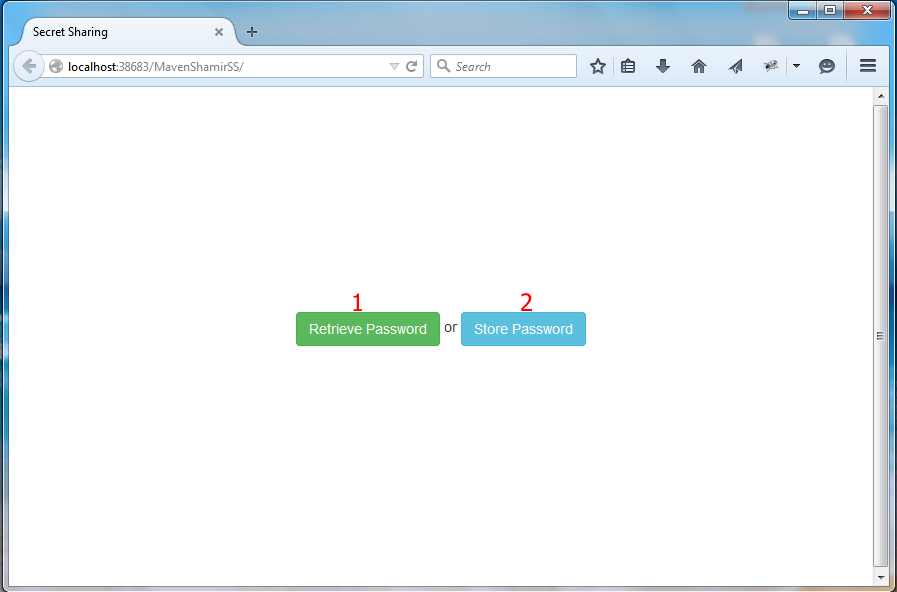
\includegraphics[scale=0.5]{Gambar/tampilan1}}
	\caption{Tampilan antarmuka awal}\label{fig:tampilan1}
\end{figure}

Setelah tombol \textit{"Store Password"} ditekan, tampilan antarmuka perangkat lunak akan terlihat seperti pada Gambar \ref{fig:tampilan2} dengan keterangan sebagai berikut.

\begin{itemize}
	\item Bagian nomor 3 merupakan tombol untuk menambah \textit{password}. Pengguna minimal harus menambahkan 1 \textit{password}, jika tidak maka akan muncul notifikasi seperti pada Gambar \ref{fig:tampilan2_2}.
	\item Bagian nomor 4 merupakan tombol untuk menambah pertanyaan keamanan.
	\item Bagian nomor 5 merupakan tombol untuk melanjutkan menyimpan \textit{password}.
	\item Bagian nomor 6 merupakan tombol untuk kembali ke tampilan antarmuka awal.
	\item Bagian nomor 7 merupakan teks masukan untuk pertanyaan keamanan yang hendak ditambahkan.
\end{itemize}

%diagram
\begin{figure}[H]
	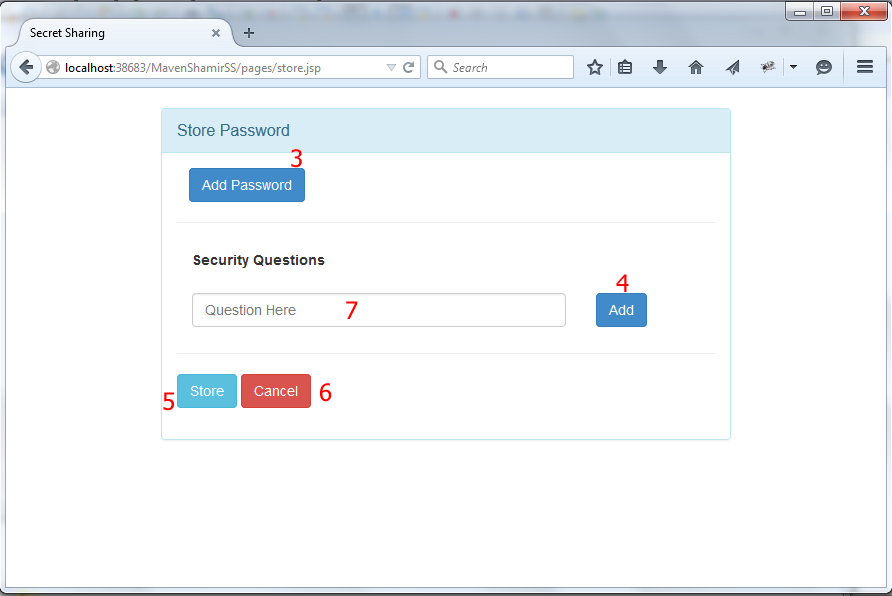
\includegraphics[scale=0.5]{Gambar/tampilan2}
	\centering
	\caption{Tampilan antarmuka untuk menyimpan \textit{password}}\label{fig:tampilan2}
\end{figure}

%diagram
\begin{figure}[H]
	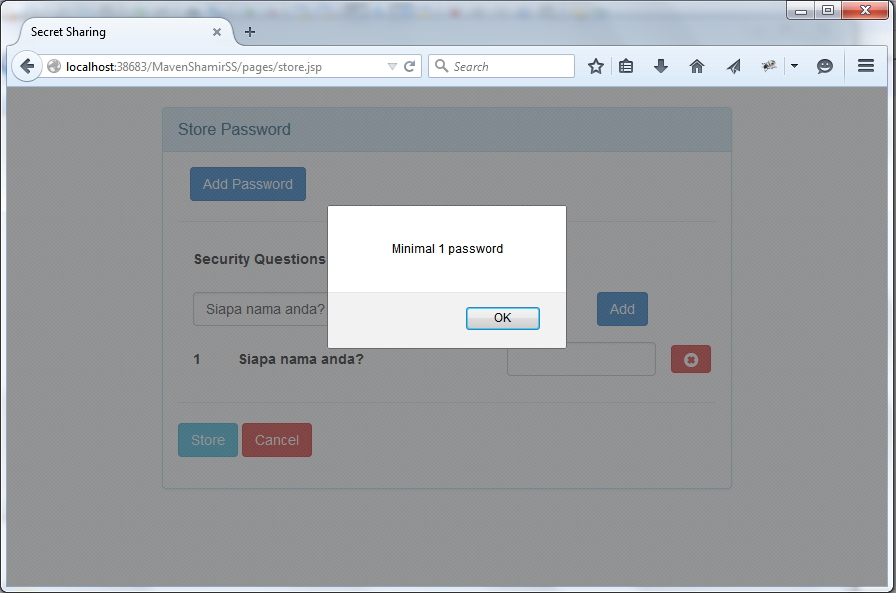
\includegraphics[scale=0.5]{Gambar/tampilan2_2}
	\centering
	\caption{Tampilan notifikasi pada antarmuka jika \textit{password} kurang}\label{fig:tampilan2_2}
\end{figure}

Setelah tombol \textit{"Add Password"} ditekan, maka tampilan antarmuka akan menambahkan masukkan teks untuk memasukkan \textit{password} yang hendak disimpan. Setelah tombol \textit{"Add"} ditekan, maka tampilan antarmuka akan menambahkan teks masukkan untuk jawaban dari pertanyaan keamanan yang sudah diisi di Bagian no 7. Tampilan yang ditunjukkan perangkat lunak dapat dilihat pada Gambar \ref{fig:tampilan2_1}.

%diagram
\begin{figure}[H]
	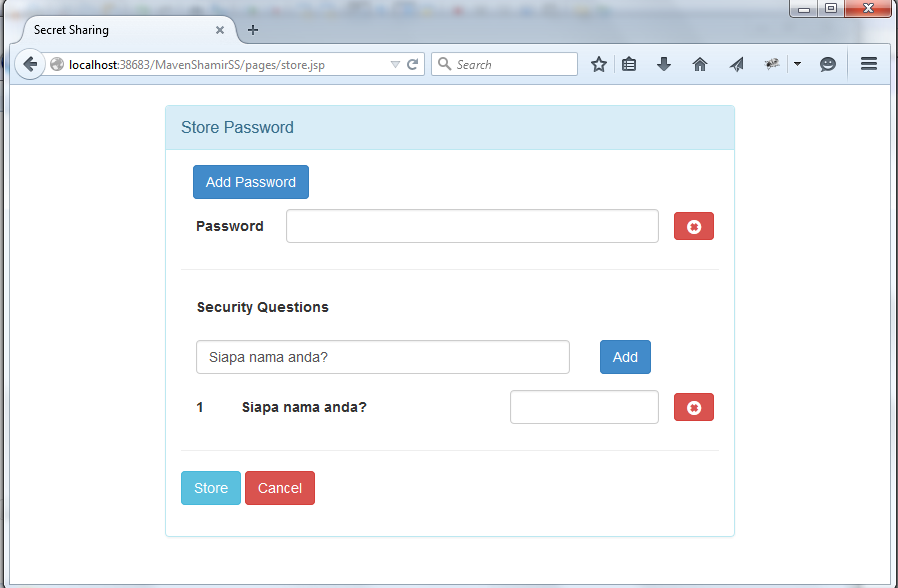
\includegraphics[scale=0.5]{Gambar/tampilan2_1}
	\centering
	\caption{Tampilan antarmuka menambah \textit{password}}\label{fig:tampilan2_1}
\end{figure}

Setelah tombol \textit{"Store"} ditekan, maka tampilan antarmuka perangkat lunak akan kembali ke tampilan antarmuka awal. \textit{Password} sudah berhasil disimpan. Kemudian, setelah tombol \textit{"Retrieve Password"} ditekan, maka tampilan perangkat lunak akan terlihat seperti pada Gambar \ref{fig:tampilan3} dengan keterangan sebagai berikut.

\begin{itemize}
	\item Bagian nomor 8 merupakan bagian dari pertanyaan keamanan yang harus dijawab oleh pengguna.
	\item Bagian nomor 9 merupakan bagian dari jawaban setiap pertanyaan keamanan yang harus dijawab.
	\item Bagian nomor 10 merupakan tombol untuk mengembalikan \textit{password}.
	\item Bagian nomor 11 merupakan tombol untuk kembali ke tampilan antarmuka awal.
\end{itemize}

%diagram
\begin{figure}[H]
	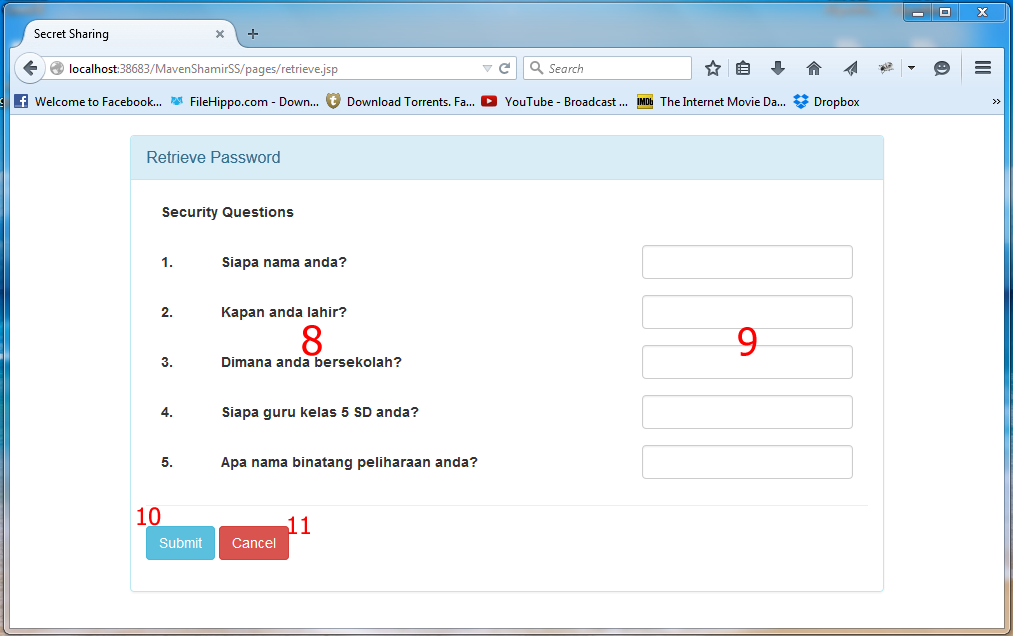
\includegraphics[scale=0.5]{Gambar/tampilan3}
	\centering
	\caption{Tampilan antarmuka untuk mengembalikan \textit{password}}\label{fig:tampilan3}
\end{figure}

Setelah tombol "Submit" pada Gambar \ref{fig:tampilan3} ditekan, perangkat lunak akan memroses setiap pertanyaan dan jawaban. Jika banyak jawaban benar dari pertanyaan keamanan yang dijawab oleh pengguna sesuai dengan minimal banyak pertanyaan keamanan yang dijawab benar yang sudah ditentukan sebelumnya, maka tampilan perangkat lunak akan terlihat seperti pada Gambar \ref{fig:tampilan4}.

%diagram
\begin{figure}[H]
	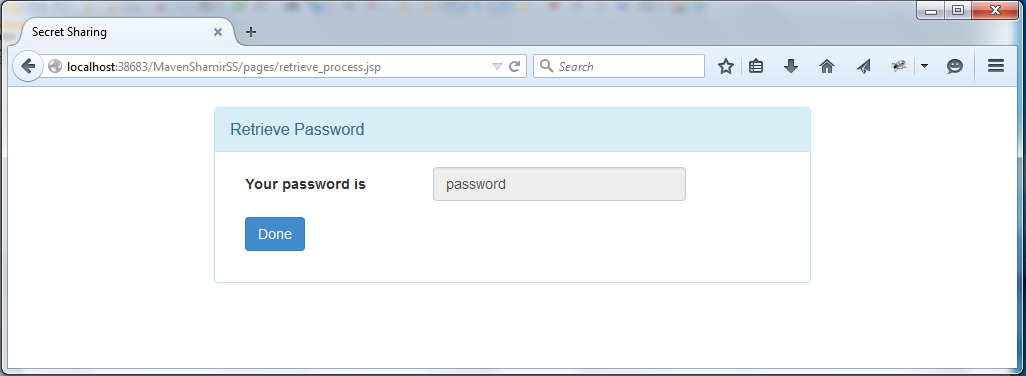
\includegraphics[scale=0.5]{Gambar/tampilan4}
	\centering
	\caption{Tampilan antarmuka untuk mengembalikan \textit{password} (2)}\label{fig:tampilan4}
\end{figure}

Sedangkan, jika pertanyaan keamanan yang dijawab benar kurang dari minimal pertanyaan keamanan yang harus dijawab benar, maka tampilan perangkat lunak akan menunjukkan notifikasi bahwa \textit{password} tidak bisa dikembalikan. Gambar \ref{fig:tampilan4_1} menunjukkan tampilan antarmuka perangkat lunak dengan notifikasi \textit{password} tidak bisa dikembalikan.

%diagram
\begin{figure}[H]
	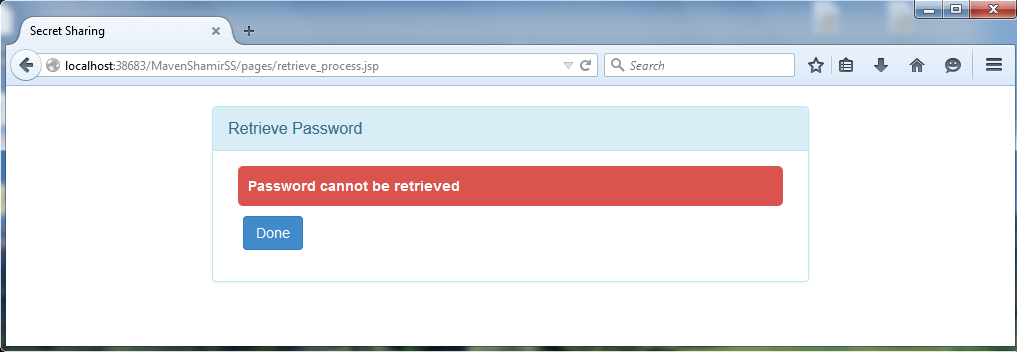
\includegraphics[scale=0.5]{Gambar/tampilan4_1}
	\centering
	\caption{Tampilan antarmuka untuk mengembalikan \textit{password} (3)}\label{fig:tampilan4_1}
\end{figure}

\section{Pengujian Perangkat Lunak}

Pada bagian ini akan berisi tentang metode pengujian, hasil pengujian, analisis pengujian, dan kesimpulan dari pengujian perangkat lunak yang sudah dibangun.

\subsection{Metode Pengujian}

Pengujian terhadap perangkat lunak yang sudah dibangun akan dibagi menjadi 2 bagian, yaitu pengujian fungsional dan pengujian suvei. Pada bagian ini akan dijelaskan masing-masing dari pengujian dan kasus yang akan digunakan dalam masing-masing pengujian yang dilakukan.

\subsubsection{Pengujian Fungsional}
	
Pengujian fungsional bertujuan untuk menguji apakah perangkat lunak dapat berfungsi sesuai dengan harapan. Dalam penelitian ini, perangkat lunak yang dibangun diharapkan dapat menyimpan \textit{password} dalam bentuk \textit{share-share} dan bisa mengembalikan banyak \textit{password} sekaligus dengan menjawab beberapa pertanyaan keamanan.

Kasus yang digunakan dalam pengujian fungsional terdiri dari 2 kasus. Kasus pertama adalah kasus dimana jika sebagian besar pertanyaan keamanan dapat dijawab dengan benar maka password akan bisa dikembalikan. Kasus kedua adalah kasus dimana jika pertanyaan keamanan yang dijawab benar tidak mencapai minimal pertanyaan keamanan yang dijawab benar sehingga password tidak bisa dikembalikan.

\subsubsection{Pengujian Survei}

Pengujian survei bertujuan untuk menguji kualitas dari pertanyaan keamanan yang dibuat saat proses menyimpan \textit{password}. Pengujian survei akan menguji pertanyaan keamanan dibuat berpengaruh pada mudah atau tidaknya password bisa dikembalikan. Setiap pertanyaan ini akan dikelompokkan menjadi beberapa topik kasus yang sesuai dengan jenisnya.

Kasus yang digunakan dalam terdiri dari 4 kasus yang masing-masing terbagi atas topiknya masing-masing. Berikut penjelasan masing-masing topik kasus.

\begin{enumerate}[itemsep=0mm]
	\item Topik 1 \\
	Pertanyaan keamanan yang kemungkinan jawabannya hanya 2, yaitu Ya atau Tidak. Selain itu, dalam topik ini digunakan pertanyaan keamanan yang jawabannya bisa dicari di \textit{internet} atau media sosial.
	\item Topik 2 \\
	Pertanyaan keamanan yang sebagian besar jawabannya mengenai angka, seperti tanggal, bulan, tahun, dan sebagainya.
	\item Topik 3 \\
	Pertanyaan keamanan yang jawabannya mengenai hal-hal personal.
	\item Topik 4 \\
	Topik 4 akan berisi gabungan dari topik 1, topik 2, dan topik 3.
\end{enumerate}

\subsection{Hasil Pengujian Fungsional}\label{subsec:hasil_pengujian_fungsional}

Sebelum dibahas hasil pengujian terhadap kasus-kasus yang sudah dijelaskan pada bagian metode pengujian fungsional, langkah pertama yang harus dilakukan adalah menyimpan \textit{password}. Untuk pengujian fungsional ini, $n$ yang dipilih adalah $n=5$ dan $k$ yang dipilih adalah $k=4$. Karena itu, ada 5 \textit{password} yang akan disimpan dan ada 5 pertanyaan keamanan yang dibuat untuk masing-masing \textit{password}. Langkah ini ditunjukkan pada Gambar \ref{fig:simpan_password}.

%diagram
\begin{figure}[H]
	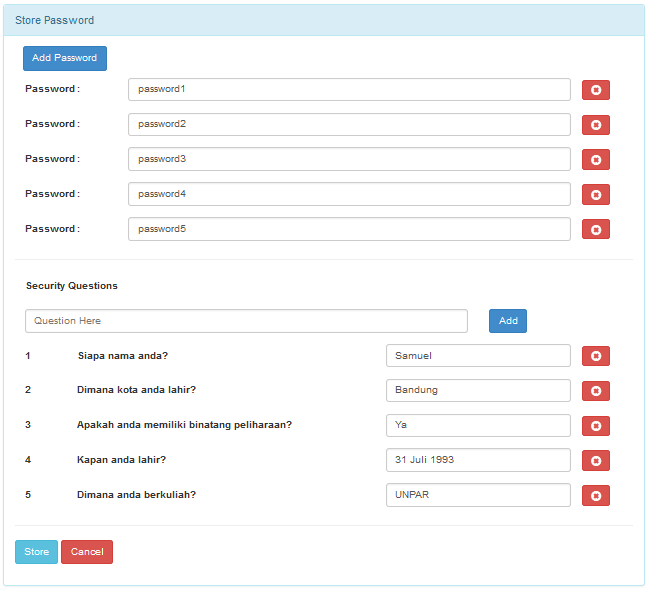
\includegraphics[scale=0.8]{Gambar/simpan_password}
	\centering
	\caption{Langkah menyimpan \textit{password}}\label{fig:simpan_password}
\end{figure}

Masukan password akan pada Gambar \ref{fig:simpan_password} ditunjukkan hanya sebagai bagian dari pengujian saja. Selanjutnya, setelah tombol "\textit{Store}" ditekan, maka password akan disimpan dan tampilan antarmuka perangkat lunak akan kembali ke tampilan antarmuka awal. Tampilan antarmuka awal ditunjukkan pada Gambar \ref{fig:tampilan1}.

Sesudah menyimpan password, langkah selanjutnya adalah melakukan pengujian terhadap kasus-kasus yang sudah dibahas pada bagian sebelumnya. Kasus pertama dari pengujian fungsional adalah kasus pertanyaan yang dijawab dengan benar sebanyak nilai $k$ atau lebih. Hasil yang diharapkan dari kasus pertama adalah password bisa dikembalikan karena banyak pertanyaan yang dijawab dengan benar sebanyak nilai $k$ atau lebih.

Langkah pertama yang perlu dilakukan dalam pengujian terhadap kasus-kasus adalah menjawab pertanyaan keamanan yang sudah disimpan. Untuk bisa menjawab pertanyaan keamanan yang sudah disimpan, tombol "\textit{Retrieve Password}" pada tampilan antarmuka awal harus ditekan. Setelah tombol tersebut ditekan, perangkat lunak akan menampilan tampilan pada Gambar \ref{fig:fungsional1}. Setiap pertanyaan pada Gambar \ref{fig:fungsional1} dijawab dengan mengisi masukan teks yang ada di samping masing-masing pertanyaan keamanan.

%diagram
\begin{figure}[H]
	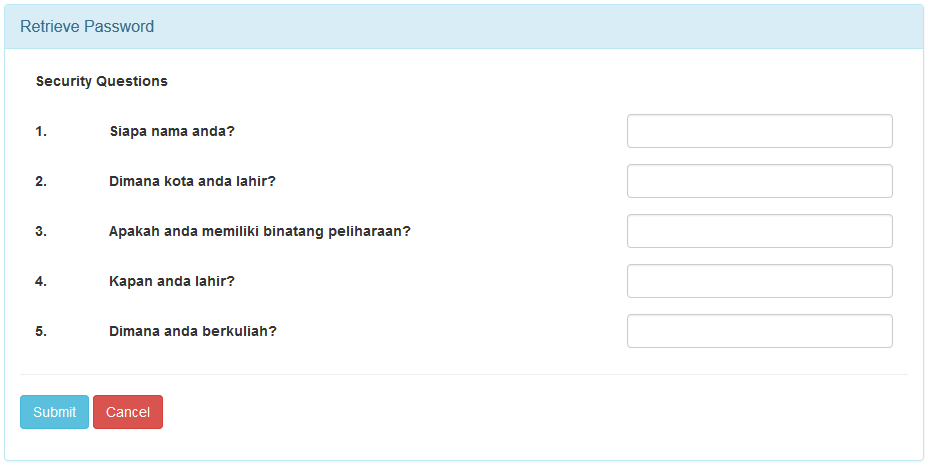
\includegraphics[scale=0.6]{Gambar/fungsional1}
	\centering
	\caption{Tampilan Menjawab Pertanyaan Keamanan}\label{fig:fungsional1}
\end{figure}

\subsubsection{Kasus 1}

Dalam kasus pertama, hasil yang diharapkan adalah password bisa dikembalikan. Maka dari itu, masukan teks ini akan diisi dengan jawaban yang benar dari masing-masing pertanyaan. Gambar \ref{fig:fungsional2} menunjukkan masukan teks yang sudah diisi dengan jawaban yang benar dari masing-masing pertanyaan.

%diagram
\begin{figure}[H]
	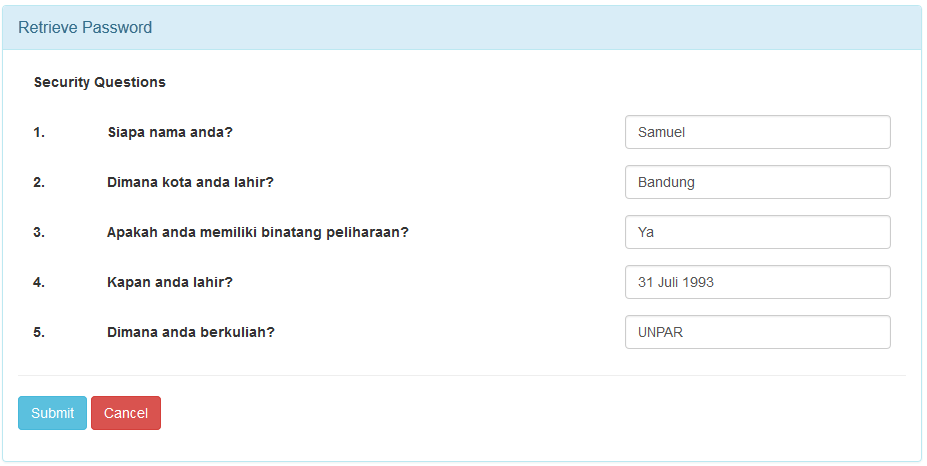
\includegraphics[scale=0.6]{Gambar/fungsional2}
	\centering
	\caption{Tampilan Menjawab Pertanyaan Keamanan Kasus Pertama}\label{fig:fungsional2}
\end{figure}

Setelah mengisi jawaban untuk masing-masing pertanyaan, langkah berikutnya adalah memroses jawaban dari masing-masing pertanyaan ini dengan metode skema threshold(k, n) yang sudah dibahas pada Bab \ref{sec:secretsharingshamir}. Untuk memroses hal ini, maka tombol "\textit{Submit}" pada Gambar \ref{fig:fungsional2} perlu ditekan.

Setelah tombol "Submit" pada Gambar \ref{fig:fungsional2} ditekan, perangkat lunak akan memroses setiap jawaban masing-masing pertanyaan. Dalam kasus pertama, seluruh pertanyaan bisa dijawab dengan benar, maka \textit{password} bisa dikembalikan. Gambar \ref{fig:fungsional3} menunjukkan bahwa \textit{password} bisa dikembalikan.

%diagram
\begin{figure}[H]
	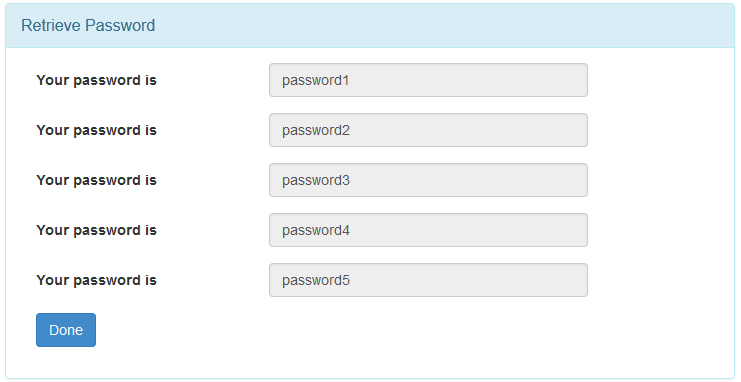
\includegraphics[scale=0.7]{Gambar/fungsional3}
	\centering
	\caption{Hasil Pengujian Fungsional Kasus Pertama}\label{fig:fungsional3}
\end{figure}

\subsubsection{Kasus 2}

Kasus selanjutnya adalah kasus kedua dimana \textit{password} tidak bisa dikembalikan. Dalam kasus ini, diasumsikan hanya 3 pertanyaan saja yang bisa dijawab dengan benar. Gambar \ref{fig:fungsional4} menunjukkan tampilan menjawab pertanyaan untuk kasus 2.

%diagram
\begin{figure}[H]
	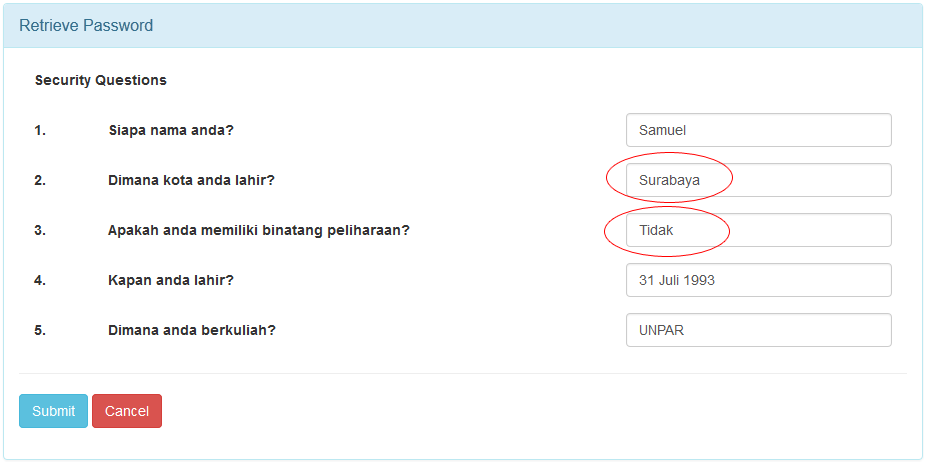
\includegraphics[scale=0.6]{Gambar/fungsional4}
	\centering
	\caption{Tampilan Menjawab Pertanyaan Keamanan Kasus Kedua}\label{fig:fungsional4}
\end{figure}

Pada Gambar \ref{fig:fungsional4} dapat dilihat bahwa hanya ada 3 pertanyaan yang dijawab dengan benar. Pertanyaan nomor 2 dan 3 diberi tanda untuk menunjukkan bahwa jawaban dari pertanyaan tersebut tidak tepat.

Langkah selanjutnya adalah memroses jawaban dari masing-masing pertanyaan dengan menekan tombol "\textit{Submit}". Setelah tombol "\textit{Submit}" ditekan, perangkat lunak akan menampilkan hasil pengujian kasus kedua. Dalam kasus kedua, karena $k$ yang dipilih $k=4$ dan hanya 3 pertanyaan yang dijawab dengan benar, maka \textit{password} tidak bisa dikembalikan. Gambar \ref{fig:fungsional5} menunjukkan langkah yang sudah dijelaskan.

%diagram
\begin{figure}[H]
	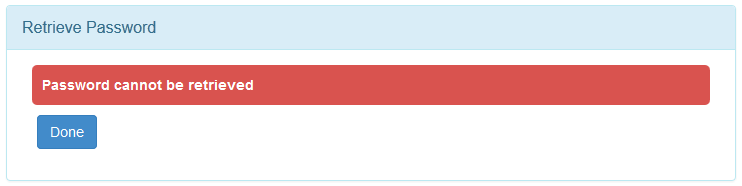
\includegraphics[scale=0.7]{Gambar/fungsional5}
	\centering
	\caption{Hasil Pengujian Fungsional Kasus Kedua}\label{fig:fungsional5}
\end{figure}

\subsection{Analisis Hasil Pengujian Fungsional}

Pada bagian ini akan dibahas analisis dari hasil pengujian fungsional yang sudah dilakukan. Seperti yang sudah dibahas, pengujian fungsional dibagi menjadi 2 kasus, yaitu kasus \textit{password} bisa dikembalikan dan kasus dimana \textit{password} tidak bisa dikembalikan.

Untuk kasus pertama, dapat dilihat bahwa jika pertanyaan keamanan yang dijawab benar lebih besar atau sama dengan nilai $k$ yang sudah ditentukan, maka semua password bisa dikembalikan. Dalam kasus pertama, seluruh pertanyaan dapat dijawab dengan benar, $pertanyaan benar = 5$. Kemudian untuk kasus pertama, nilai $k=4$ dan $pertanyaan benar > k$. Maka dari itu, \textit{password} bisa dikembalikan.

Untuk kasus kedua, dapat dilihat bahwa jika pertanyaan keamanan yang dijawab benar kurang dari $k$, maka password tidak bisa dikembalikan. Dalam kasus kedua, banyak pertanyaan yang dijawab benar hanya 3 pertanyaan, $pertanyaan benar=3$. Jadi, karena $k=4$ dan $pertanyaan benar < k$, \textit{password} tidak bisa dikembalikan.

Jadi, kesimpulan yang dapat diambil dari hasil pengujian kasus pertama dan kedua adalah perangkat lunak sudah bisa mengimplementasikan metode \textit{secret sharing} Shamir untuk mengembalikan $n$ password dengan menjawab $n$ pertanyaan.

\subsection{Analisis dan Hasil Pengujian Survei}\label{subsec:hasil_pengujian_survei}

Pada bagian ini akan ditunjukkan hasil pengujian survei. Seperti yang sudah dijelaskan, pengujian survei bertujuan untuk menilai kualitas dari pertanyaan keamanan dengan melihat tingkat kesulitan untuk menebak atau menjawab jawaban benar. Asumsi yang digunakan dalam pengujian ini adalah seluruh jawaban relevan dengan pertanyaan keamanan.

Pengujian survei ini terbagi atas 4 kasus. Responden melakukan survei dengan cara mencoba untuk menebak jawaban dari pertanyaan keamanan untuk mengembalikan password. Setiap orang bebas memilih cara untuk mendapatkan jawaban dari pertanyaan selain tidak bertanya kepada pembuat pertanyaan keamanan.

Kasus 1, 2, dan 3 memiliki 10 pertanyaan keamanan, $n=10$, dan minimal 4 pertanyaan keamanan dijawab benar, $k=4$. Sementara itu, untuk kasus 4 nilai $n$ dan $k$ ditambah. Dalam kasus 4, terdapat 15 pertanyaan keamanan, $n=15$, dan minimal 6 pertanyaan keamanan dijawab benar, $k=6$. Berikut tabel hasil survei untuk setiap kasus beserta dengan penjelasannya. Untuk kasus 1 dan 2 survei dilakukan terhadap 7 orang responden, sedangkan untuk kasus 3 dan 4 survei dilakukan terhadap 20 orang responden.

\subsubsection{Kasus 1}

Berikut daftar pertanyaan keamanan yang digunakan dalam kasus 1:

\begin{enumerate}[itemsep=0mm]
	\item Apa jenis kelamin anda? (Laki-laki/Perempuan)
	\item Apakah anda pernah ke luar negeri?
	\item Apakah anda mempunyai binatang peliharaan?
	\item Apakah anda bermain alat musik?
	\item Apakah anda pernah tidak naik kelas?
	\item Apakah anda pernah mengalami kecelakaan?
	\item Apakah anda menyukai kegiatan olahraga?
	\item Apa nama belakang anda?
	\item Siapa nama ibu anda?
	\item Siapa nama ayah anda?
\end{enumerate}

Kemudian, hasil dari survei kasus 1 ditunjukkan oleh Grafik \ref{fig:kasus1}.

%diagram
\begin{figure}[H]
	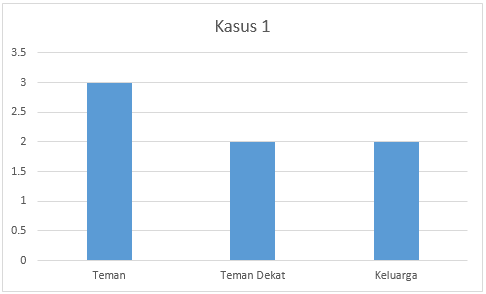
\includegraphics[scale=0.8]{Gambar/kasus1}
	\centering
	\caption{Pengujian survei kasus 1}\label{fig:kasus1}
\end{figure}

\subsubsection{Analisis Kasus 1}

Dilihat dari grafik \ref{fig:kasus1} untuk topik kasus 1, seluruh responden bisa berhasil mengembalikan \textit{password}. Hal ini karena mayoritas kemungkinan jawaban dari pertanyaan keamanan adalah kemungkinan biner dengan hanya 2 kemungkinan saja (Ya atau Tidak). Pertanyaan keamanan yang kemungkinan jawabannya hanya 2 kemungkinan saja bisa dengan mudah ditebak. Karena setiap jawaban bisa dengan mudah ditebak, maka seluruh responden bisa mengembalikan \textit{password} dengan mudah.

\subsubsection{Kasus 2}

Berikut daftar pertanyaan keamanan yang digunakan dalam kasus 2:

\begin{enumerate}[itemsep=0mm]
	\item Pada tahun berapa anda lahir?
	\item Pada tanggal berapa anda lahir?
	\item Pada bulan apa anda lahir?
	\item Berapa perbedaan umur anda dengan ayah anda?
	\item Berapa perbedaan umur anda dengan ibu anda?
	\item Berapa orang saudara anda?
	\item Berapa nomor rumah tempat anda tinggal?
	\item Dimana anda tinggal?
	\item Apa merek kendaraan yang anda pakai?
	\item Pada hari apa anda lahir?
\end{enumerate}

Kemudian, hasil dari survei kasus 2 ditunjukkan oleh Grafik \ref{fig:kasus2}.

%diagram
\begin{figure}[H]
	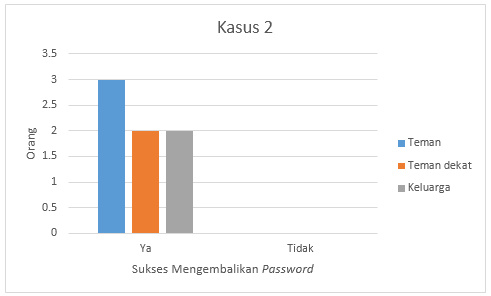
\includegraphics[scale=0.8]{Gambar/kasus2}
	\centering
	\caption{Pengujian survei kasus 2}\label{fig:kasus2}
\end{figure}

\subsubsection{Analisis Kasus 2}

Dilihat dari grafik \ref{fig:kasus2} untuk topik kasus 2, seluruh responden berhasil untuk mengembalikan password. Hal ini disebabkan karena kemungkinan jawaban dari pertanyaan keamanan hanya berupa angka saja, khususnya hanya tanggal ulang tahun, bulan lahir, atau tahun lahir.

Responden dapat menjawab tanggal lahir karena hanya memiliki 30-31 kemungkinan, sedangkan untuk bulan hanya ada 12 kemungkinan, dan juga beberapa pertanyaan lain yang menyangkut angka. Dapat dilihat juga, bahwa beberapa jawaban untuk pertanyaan keamanan merupakan informasi yang sering ditunjukkan dalam profil sosial media, karena dari itu jawaban yang tepat bisa dengan mudah didapatkan.

\subsubsection{Kasus 3}

Berikut daftar pertanyaan keamanan yang digunakan dalam kasus 3:

\begin{enumerate}[itemsep=0mm]
	\item Pada jam berapa anda lahir?(jj:mm)
	\item Apa nama sekolah dasar tempat anda bersekolah?
	\item Siapa nama belakang sepupu paling tua dari keluarga sisi ibu anda?
	\item Siapa nama belakang sepupu paling tua dari keluarga sisi ayah anda?
	\item Apa cita-cita anda dulu sewaktu kecil?
	\item Siapa nama anak paling tua dari nenek sisi ibu anda?
	\item Apa binatang peliharaan pertama anda?
	\item Apa alat musik yang anda mainkan pertama kali?
	\item Dimana kerabat terdekat anda tinggal/berasal?
	\item Siapa nama guru kelas 3 SD anda?
\end{enumerate}

Kemudian, hasil dari survei kasus 3 ditunjukkan oleh Grafik \ref{fig:kasus3}.

%diagram
\begin{figure}[H]
	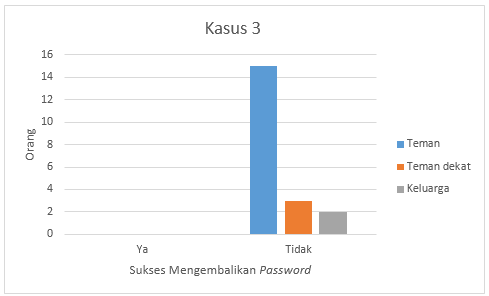
\includegraphics[scale=0.8]{Gambar/kasus3}
	\centering
	\caption{Pengujian survei kasus 3}\label{fig:kasus3}
\end{figure}

\subsubsection{Analisis Kasus 3}

Untuk topik kasus 3, tidak ada responden yang berhasil mengembalikan \textit{password}. Hal ini karena beberapa pertanyaan sifatnya sangat personal dan jawaban tidak bisa dengan mudah ditebak atau dicari di \textit{internet} atau media sosial. Pertanyaan yang sifatnya sangat personal akan mempersulit untuk mengembalikan \textit{password} kecuali bagi pembuat pertanyaan.

\subsubsection{Kasus 4}

Berikut daftar pertanyaan keamanan yang digunakan dalam kasus 4:

\begin{enumerate}[itemsep=0mm]
	\item Apakah anda mempunyai binatang peliharaan?
	\item Apakah anda bermain alat musik?
	\item Apakah anda pernah tidak naik kelas?
	\item Apa nama belakang anda?
	\item Siapa nama ibu anda?
	\item Pada hari apa anda lahir?
	\item Pada tanggal berapa anda lahir?
	\item Pada bulan apa anda lahir?
	\item Berapa perbedaan umur anda dengan ayah anda?
	\item Berapa nomor rumah tempat anda tinggal?
	\item Pada jam berapa anda lahir?(jj:mm)
	\item Apa cita-cita anda dulu sewaktu kecil?
	\item Siapa nama anak paling tua dari nenek sisi ibu anda?
	\item Apa binatang peliharaan pertama anda?
	\item Siapa nama guru kelas 3 SD anda?
\end{enumerate}

Kemudian, Grafik \ref{fig:kasus4} menunjukkan hasil survei kasus 4.

%diagram
\begin{figure}[H]
	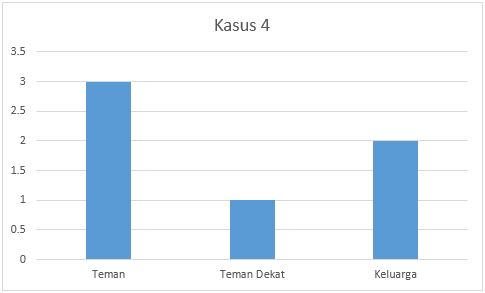
\includegraphics[scale=0.8]{Gambar/kasus4}
	\centering
	\caption{Pengujian survei kasus 4}\label{fig:kasus4}
\end{figure}

\subsubsection{Analisis Kasus 4}

Dilihat dari grafik \ref{fig:kasus4} untuk topik kasus 4, tingkat keberhasilannya tetap tinggi walaupun topik kasus 4 ini merupakan gabungan dari topik kasus 1, 2, dan 3. Hal ini disebabkan karena mayoritas terdiri pertanyaan dari kasus 1 dan kasus 2.

Responden hanya cukup menjawab 6 pertanyaan benar dari 15 pertanyaan dalam kasus 4, maka responden pun cukup menjawab 3 pertanyaan dari kasus 1 dan 3 pertanyaan dari kasus 2 dengan benar, responden tidak perlu menjawab satupun pertanyaan dari kasus 3. Dapat disimpulkan, bahwa meningkatkan banyak pertanyaan keamanan tidak mempersulit untuk mengembalikan \textit{password}.

\subsection{Kesimpulan Pengujian}

Dari 4 kasus pengujian yang dilakukan maka bisa ditarik beberapa kesimpulan dalam penilaian kualitas pertanyaan keamanan personal. Pertanyaan keamanan personal harus memiliki 5 sifat:
\begin{itemize}
	\item Aman \\
	Pertanyaan keamanan harus tidak mudah ditebak dan tidak mudah diselidiki (\textit{googling}).
	\item Stabil \\
	Pertanyaan keamanan tidak boleh berubah seiring berjalannya waktu.
	\item Mudah diingat \\
	Pertanyaan keamanan harus sifatnya personal sehingga mudah untuk diingat.
	\item Sederhana \\
	Pertanyaan keamanan harus sederhana tetapi sifatnya tetap personal.
	\item Memiliki banyak kemungkinan jawaban \\
	Pertanyaan keamanan tidak boleh hanya memiliki kemungkinan jawaban yang sedikit karena akan mudah ditebak (dengan teknik \textit{brute force}).
\end{itemize}

Namun, beberapa pertanyaan keamanan mungkin memiliki banyak kemungkinan jawaban dan aman sehingga tidak mudah ditebak tetapi tidak mudah diingat karena jawabannya terlalu rumit. Beberapa pertanyaan keamanan juga mungkin tidak sesuai dengan situasi atau keadaan dari pembuat pertanyaan. Sehingga, tidak ada pertanyaan keamanan yang memiliki tepat 5 sifat yang diatas.